\documentclass[tikz,dvipdfmx,dvipsnames]{standalone}

\usepackage{amsmath, amssymb, amsthm, mathrsfs, amsfonts, dsfont}
\usepackage{bbm}
\usepackage{bm}
\usepackage{physics}
\usepackage{ifthen}
\usepackage{setspace}
\usepackage{mathtools}

\newcommand{\defeq}{\coloneqq}

\newcommand{\red}[1]{\textcolor{red}{#1}}
\newcommand{\blue}[1]{\textcolor{blue}{#1}}
\newcommand{\cyan}[1]{\textcolor{cyan}{#1}}
\newcommand{\gray}[1]{\textcolor{gray}{#1}}
\newcommand{\green}[1]{\textcolor{green}{#1}}
\newcommand{\brown}[1]{\textcolor{brown}{#1}}
\newcommand{\black}[1]{\textcolor{black}{#1}}
\newcommand{\orange}[1]{\textcolor{orange}{#1}}
\newcommand{\purple}[1]{\textcolor{purple}{#1}}
\newcommand{\yellow}[1]{\textcolor{yellow}{#1}}
\newcommand{\Magenta}[1]{\textcolor{Magenta}{#1}}
\newcommand{\RoyalBlue}[1]{\textcolor{RoyalBlue}{#1}}
\newcommand{\RubineRed}[1]{\textcolor{RubineRed}{#1}}
\newcommand{\ForestGreen}[1]{\textcolor{ForestGreen}{#1}}
\newcommand{\YellowOrange}[1]{\textcolor{YellowOrange}{#1}}
\newcommand{\WildStrawberry}[1]{\textcolor{WildStrawberry}{#1}}

\usetikzlibrary{calc,matrix,math}
\usetikzlibrary{decorations.pathreplacing,calligraphy,shapes.arrows}

\definecolor{c0}{RGB}{253, 231, 36}
\definecolor{c1}{RGB}{154, 216, 60}
\definecolor{c2}{RGB}{91, 200, 98}
\definecolor{c3}{RGB}{59, 81, 138}
\definecolor{c4}{RGB}{69, 50, 127}

\begin{document}

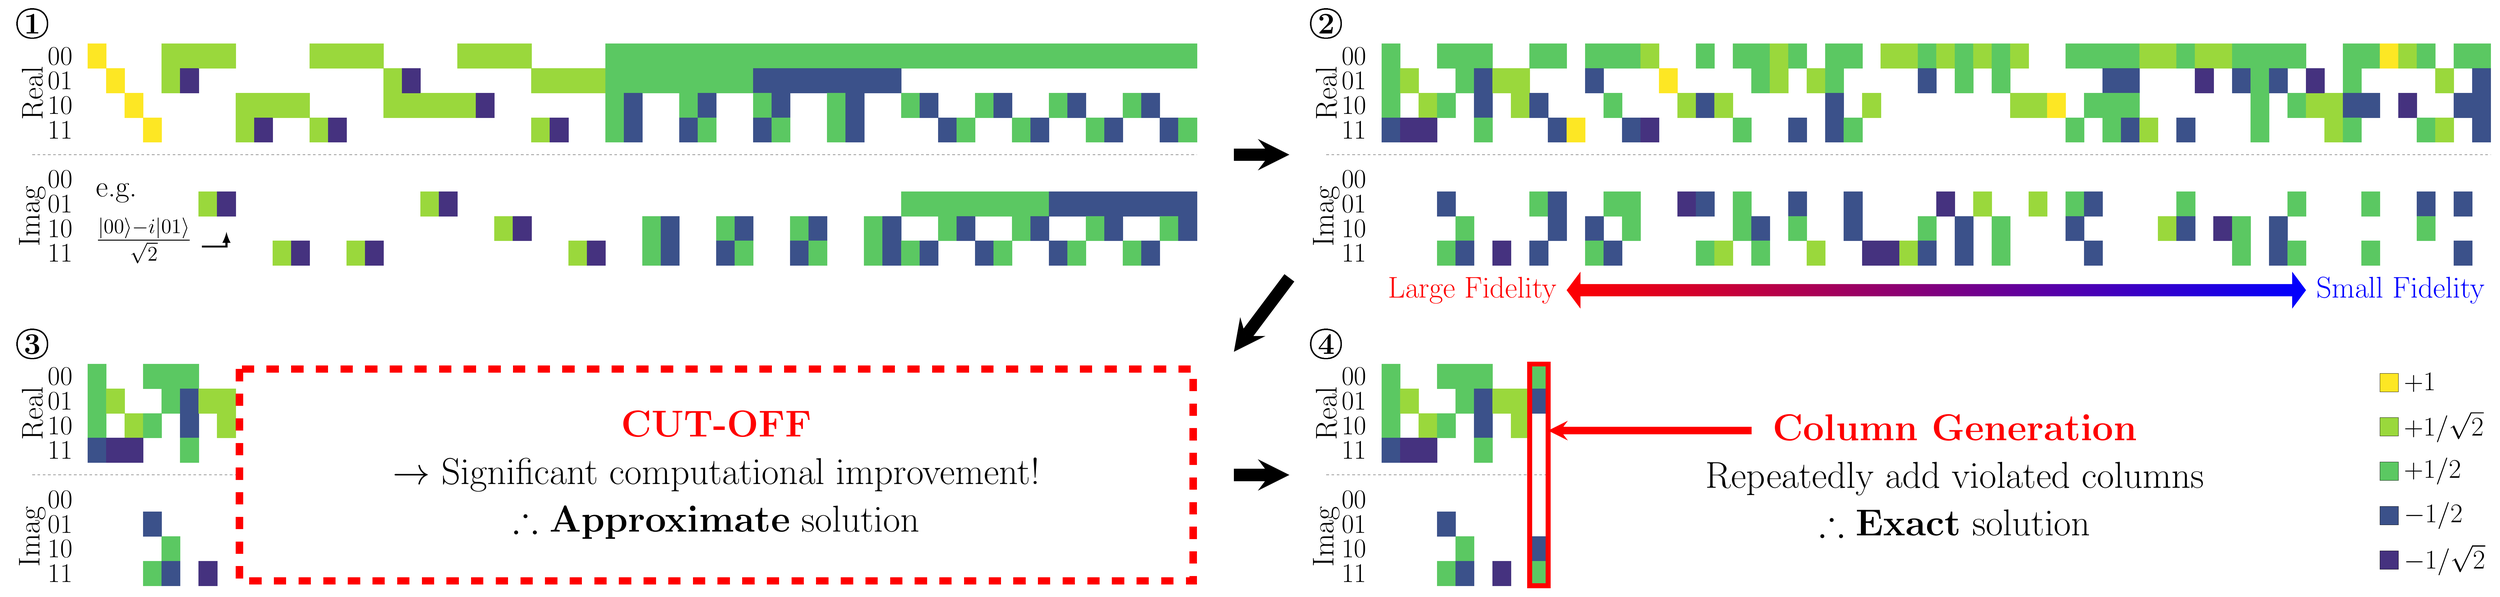
\begin{tikzpicture}[xscale=0.75]
    \begin{scope}[yscale=0.75,xshift=124cm,yshift=-13*1.333333cm]
        \draw[fill=c0] (0, 0.7-1*1.2) rectangle (1, 0.7-1*1.2-1);
        \draw[fill=c1] (0, 0.7-3*1.2) rectangle (1, 0.7-3*1.2-1);
        \draw[fill=c2] (0, 0.7-5*1.2) rectangle (1, 0.7-5*1.2-1);
        \draw[fill=c3] (0, 0.7-7*1.2) rectangle (1, 0.7-7*1.2-1);
        \draw[fill=c4] (0, 0.7-9*1.2) rectangle (1, 0.7-9*1.2-1);
        \node[anchor=west,font=\LARGE,scale=1.8] at (1, 0.7-1*1.2-0.5) {$+1$};
        \node[anchor=west,font=\LARGE,scale=1.8] at (1, 0.7-3*1.2-0.5) {$+1/\sqrt{2}$};
        \node[anchor=west,font=\LARGE,scale=1.8] at (1, 0.7-5*1.2-0.5) {$+1/2$};
        \node[anchor=west,font=\LARGE,scale=1.8] at (1, 0.7-7*1.2-0.5) {$-1/2$};
        \node[anchor=west,font=\LARGE,scale=1.8] at (1, 0.7-9*1.2-0.5) {$-1/\sqrt{2}$};
    \end{scope}

    \begin{scope}
        \foreach \color/\col/\row in {
                c0/0/0,
                c0/1/-1,
                c0/2/-2,
                c0/3/-3,
                c1/4/0,
                c1/4/-1,
                c1/5/0,
                c4/5/-1,
                c1/6/0,
                c1/6/-6,
                c1/7/0,
                c4/7/-6,
                c1/8/-2,
                c1/8/-3,
                c1/9/-2,
                c4/9/-3,
                c1/10/-2,
                c1/10/-8,
                c1/11/-2,
                c4/11/-8,
                c1/12/0,
                c1/12/-3,
                c1/13/0,
                c4/13/-3,
                c1/14/0,
                c1/14/-8,
                c1/15/0,
                c4/15/-8,
                c1/16/-2,
                c1/16/-1,
                c1/17/-2,
                c4/17/-1,
                c1/18/-2,
                c1/18/-6,
                c1/19/-2,
                c4/19/-6,
                c1/20/0,
                c1/20/-2,
                c1/21/0,
                c4/21/-2,
                c1/22/0,
                c1/22/-7,
                c1/23/0,
                c4/23/-7,
                c1/24/-1,
                c1/24/-3,
                c1/25/-1,
                c4/25/-3,
                c1/26/-1,
                c1/26/-8,
                c1/27/-1,
                c4/27/-8,
                c2/28/0,
                c2/28/-1,
                c2/28/-2,
                c2/28/-3,
                c2/29/0,
                c2/29/-1,
                c3/29/-2,
                c3/29/-3,
                c2/30/0,
                c2/30/-1,
                c2/30/-7,
                c2/30/-8,
                c2/31/0,
                c2/31/-1,
                c3/31/-7,
                c3/31/-8,
                c2/32/0,
                c2/32/-1,
                c2/32/-2,
                c3/32/-3,
                c2/33/0,
                c2/33/-1,
                c3/33/-2,
                c2/33/-3,
                c2/34/0,
                c2/34/-1,
                c2/34/-7,
                c3/34/-8,
                c2/35/0,
                c2/35/-1,
                c3/35/-7,
                c2/35/-8,
                c2/36/0,
                c3/36/-1,
                c2/36/-2,
                c3/36/-3,
                c2/37/0,
                c3/37/-1,
                c3/37/-2,
                c2/37/-3,
                c2/38/0,
                c3/38/-1,
                c2/38/-7,
                c3/38/-8,
                c2/39/0,
                c3/39/-1,
                c3/39/-7,
                c2/39/-8,
                c2/40/0,
                c3/40/-1,
                c2/40/-2,
                c2/40/-3,
                c2/41/0,
                c3/41/-1,
                c3/41/-2,
                c3/41/-3,
                c2/42/0,
                c3/42/-1,
                c2/42/-7,
                c2/42/-8,
                c2/43/0,
                c3/43/-1,
                c3/43/-7,
                c3/43/-8,
                c2/44/0,
                c2/44/-6,
                c2/44/-2,
                c2/44/-8,
                c2/45/0,
                c2/45/-6,
                c3/45/-2,
                c3/45/-8,
                c2/46/0,
                c2/46/-6,
                c2/46/-7,
                c3/46/-3,
                c2/47/0,
                c2/47/-6,
                c3/47/-7,
                c2/47/-3,
                c2/48/0,
                c2/48/-6,
                c2/48/-2,
                c3/48/-8,
                c2/49/0,
                c2/49/-6,
                c3/49/-2,
                c2/49/-8,
                c2/50/0,
                c2/50/-6,
                c2/50/-7,
                c2/50/-3,
                c2/51/0,
                c2/51/-6,
                c3/51/-7,
                c3/51/-3,
                c2/52/0,
                c3/52/-6,
                c2/52/-2,
                c3/52/-8,
                c2/53/0,
                c3/53/-6,
                c3/53/-2,
                c2/53/-8,
                c2/54/0,
                c3/54/-6,
                c2/54/-7,
                c2/54/-3,
                c2/55/0,
                c3/55/-6,
                c3/55/-7,
                c3/55/-3,
                c2/56/0,
                c3/56/-6,
                c2/56/-2,
                c2/56/-8,
                c2/57/0,
                c3/57/-6,
                c3/57/-2,
                c3/57/-8,
                c2/58/0,
                c3/58/-6,
                c2/58/-7,
                c3/58/-3,
                c2/59/0,
                c3/59/-6,
                c3/59/-7,
                c2/59/-3
            }{
                \draw[
                    fill=\color,
                    draw=\color
                ] (\col, \row) rectangle (\col + 1, \row - 1);
            }
    \end{scope}

    \begin{scope}[xshift=70cm]
        \foreach \color/\col/\row in {
                c2/0/0,
                c2/0/-1,
                c2/0/-2,
                c3/0/-3,
                c1/1/-1,
                c4/1/-3,
                c1/2/-2,
                c4/2/-3,
                c2/3/0,
                c3/3/-6,
                c2/3/-2,
                c2/3/-8,
                c2/4/0,
                c2/4/-1,
                c2/4/-7,
                c3/4/-8,
                c2/5/0,
                c3/5/-1,
                c3/5/-2,
                c2/5/-3,
                c1/6/-1,
                c4/6/-8,
                c1/7/-2,
                c1/7/-1,
                c2/8/0,
                c2/8/-6,
                c3/8/-2,
                c3/8/-8,
                c2/9/0,
                c3/9/-6,
                c3/9/-7,
                c3/9/-3,
                c0/10/-3,
                c2/11/0,
                c3/11/-1,
                c3/11/-7,
                c2/11/-8,
                c2/12/0,
                c2/12/-6,
                c2/12/-2,
                c3/12/-8,
                c2/13/0,
                c2/13/-6,
                c2/13/-7,
                c3/13/-3,
                c1/14/0,
                c4/14/-3,
                c0/15/-1,
                c1/16/-2,
                c4/16/-6,
                c2/17/0,
                c3/17/-6,
                c3/17/-2,
                c2/17/-8,
                c1/18/-2,
                c1/18/-8,
                c2/19/0,
                c2/19/-6,
                c2/19/-7,
                c2/19/-3,
                c2/20/0,
                c2/20/-1,
                c3/20/-7,
                c2/20/-8,
                c1/21/0,
                c1/21/-1,
                c2/22/0,
                c3/22/-6,
                c2/22/-7,
                c3/22/-3,
                c1/23/-1,
                c1/23/-8,
                c2/24/0,
                c2/24/-1,
                c3/24/-2,
                c3/24/-3,
                c2/25/0,
                c3/25/-6,
                c3/25/-7,
                c2/25/-3,
                c1/26/-2,
                c4/26/-8,
                c1/27/0,
                c4/27/-8,
                c1/28/0,
                c1/28/-8,
                c2/29/0,
                c3/29/-1,
                c2/29/-7,
                c3/29/-8,
                c1/30/0,
                c4/30/-6,
                c2/31/0,
                c2/31/-1,
                c3/31/-7,
                c3/31/-8,
                c1/32/0,
                c1/32/-6,
                c2/33/0,
                c2/33/-1,
                c2/33/-7,
                c2/33/-8,
                c1/34/0,
                c1/34/-2,
                c1/35/-2,
                c1/35/-6,
                c0/36/-2,
                c2/37/0,
                c2/37/-6,
                c3/37/-7,
                c2/37/-3,
                c2/38/0,
                c3/38/-6,
                c2/38/-2,
                c3/38/-8,
                c2/39/0,
                c3/39/-1,
                c2/39/-2,
                c2/39/-3,
                c2/40/0,
                c3/40/-1,
                c2/40/-2,
                c3/40/-3,
                c1/41/0,
                c1/41/-3,
                c1/42/0,
                c1/42/-7,
                c2/43/0,
                c2/43/-6,
                c3/43/-7,
                c3/43/-3,
                c1/44/0,
                c4/44/-1,
                c1/45/0,
                c4/45/-7,
                c2/46/0,
                c3/46/-1,
                c2/46/-7,
                c2/46/-8,
                c2/47/0,
                c2/47/-1,
                c2/47/-2,
                c2/47/-3,
                c2/48/0,
                c3/48/-1,
                c3/48/-7,
                c3/48/-8,
                c2/49/0,
                c2/49/-6,
                c2/49/-2,
                c2/49/-8,
                c1/50/-2,
                c4/50/-1,
                c1/51/-2,
                c1/51/-3,
                c2/52/0,
                c2/52/-1,
                c3/52/-2,
                c2/52/-3,
                c2/53/0,
                c2/53/-6,
                c3/53/-2,
                c2/53/-8,
                c0/54/0,
                c1/55/0,
                c4/55/-2,
                c2/56/0,
                c3/56/-6,
                c2/56/-7,
                c2/56/-3,
                c1/57/-1,
                c1/57/-3,
                c2/58/0,
                c3/58/-6,
                c3/58/-2,
                c3/58/-8,
                c2/59/0,
                c3/59/-1,
                c3/59/-2,
                c3/59/-3
            }{
                \draw[
                    fill=\color,
                    draw=\color
                ] (\col, \row) rectangle (\col + 1, \row - 1);
            }
    \end{scope}

    \begin{scope}[xshift=0cm,yshift=-13cm]
        \foreach \color/\col/\row in {
                c2/0/0,
                c2/0/-1,
                c2/0/-2,
                c3/0/-3,
                c1/1/-1,
                c4/1/-3,
                c1/2/-2,
                c4/2/-3,
                c2/3/0,
                c3/3/-6,
                c2/3/-2,
                c2/3/-8,
                c2/4/0,
                c2/4/-1,
                c2/4/-7,
                c3/4/-8,
                c2/5/0,
                c3/5/-1,
                c3/5/-2,
                c2/5/-3,
                c1/6/-1,
                c4/6/-8,
                c1/7/-2,
                c1/7/-1
            }{
                \draw[
                    fill=\color,
                    draw=\color
                ] (\col, \row) rectangle (\col + 1, \row - 1);
            }
    \end{scope}

    \begin{scope}[xshift=70cm,yshift=-13cm]
        \foreach \color/\col/\row in {
                c2/0/0,
                c2/0/-1,
                c2/0/-2,
                c3/0/-3,
                c1/1/-1,
                c4/1/-3,
                c1/2/-2,
                c4/2/-3,
                c2/3/0,
                c3/3/-6,
                c2/3/-2,
                c2/3/-8,
                c2/4/0,
                c2/4/-1,
                c2/4/-7,
                c3/4/-8,
                c2/5/0,
                c3/5/-1,
                c3/5/-2,
                c2/5/-3,
                c1/6/-1,
                c4/6/-8,
                c1/7/-2,
                c1/7/-1,
                c2/8/0,
                c3/8/-1,
                c3/8/-7,
                c2/8/-8
            }{
                \draw[
                    fill=\color,
                    draw=\color
                ] (\col, \row) rectangle (\col + 1, \row - 1);
            }
    \end{scope}

    \foreach \xshiftVal/\yshifVal/\xMax in {0/0/60,70/0/60,0/-13/8,70/-13/9}{
            \begin{scope}[xshift=\xshiftVal cm,yshift=\yshifVal cm]
                \foreach \row/\label in {
                        -0.5/00,
                        -1.5/01,
                        -2.5/10,
                        -3.5/11,
                        -5.5/00,
                        -6.5/01,
                        -7.5/10,
                        -8.5/11
                    }{
                        \node[anchor=center,font=\LARGE,scale=1.8]
                        at (-1.5, \row) {\label};
                    }

                \node[anchor=center,font=\LARGE,rotate=90,scale=2]
                at (-3, -2) {Real};
                \node[anchor=center,font=\LARGE,rotate=90,scale=2]
                at (-3, -7) {Imag};

                \draw[dashed] (-3,-4.5) -- (+\xMax,-4.5);
            \end{scope}
        }


    \draw[->,>=stealth,line width=0.5cm] (62, -4.5) -- (65, -4.5);
    \draw[->,>=stealth,line width=0.5cm] (65, -9.5) -- (62, -12.5);
    \draw[->,>=stealth,line width=0.5cm] (62, -17.5) -- (65, -17.5);

    \node[font=\LARGE,scale=2,anchor=west] at ( 70,-10) { \red{Large Fidelity}};
    \node[font=\LARGE,scale=2,anchor=east] at (130,-10) {\blue{Small Fidelity}};
    \node [double arrow, left color=red, right color=blue, transform shape, minimum height=40cm,minimum width=1.5cm] at (100,-10) {};

    \draw[dashed,dash pattern=on 0.5cm off 0.5cm,red,line width=0.3cm] (8+0.2,-13-0.2) rectangle (60-0.2,-22+0.2);
    \node[font=\LARGE,scale=2.5,align=center,anchor=center] at (34,-17.5) {\red{\textbf{CUT-OFF}} \\$\rightarrow$ Significant computational improvement!\\$\therefore$ \textbf{Approximate} solution};

    \draw[red,line width=0.2cm] (78,-13) rectangle (79,-22);
    \node[font=\LARGE,scale=2.5,align=center,anchor=center] at (101,-17.5) {\red{\textbf{Column Generation}}\\Repeatedly add violated columns\\$\therefore$ \textbf{Exact} solution};
    \draw[<-,>=stealth,red,line width=0.3cm] (79,-15.7) -- (90,-15.7);

    \node[font=\LARGE,scale=2] at ( 0-3,  1-0.3) {\textbf{\textcircled{\raisebox{-2pt}{1}}}};
    \node[font=\LARGE,scale=2] at (70-3,  1-0.3) {\textbf{\textcircled{\raisebox{-2pt}{2}}}};
    \node[font=\LARGE,scale=2] at ( 0-3,-12-0.3) {\textbf{\textcircled{\raisebox{-2pt}{3}}}};
    \node[font=\LARGE,scale=2] at (70-3,-12-0.3) {\textbf{\textcircled{\raisebox{-2pt}{4}}}};

    \node[font=\LARGE,scale=2,align=left] at (4,-7.3) {e.g.\\[1ex]$\frac{\ket{00}-i\ket{01}}{\sqrt{2}}$ \tikz{\draw[-latex,very thick] (-0.5,0) -| (0,0.3);}};
\end{tikzpicture}

\end{document}